\documentclass{beamer}
\usepackage[T1]{fontenc}
\usepackage[utf8]{inputenc}
\usepackage{hyperref}
\usepackage{multimedia}
\usepackage{tabu,longtable}
\usepackage{tikz}

\mode<presentation>
\usetheme{Warsaw}
\usecolortheme{whale}

\AtBeginSection{
\begin{frame}
  \frametitle{Outline}
  \tableofcontents[currentsection]
\end{frame}
}

% for enumerate accross columns
\newcounter{savedenum}
\newcommand*{\saveenum}{\setcounter{savedenum}{\theenumi}}
\newcommand*{\resume}{\setcounter{enumi}{\thesavedenum}}

\usefonttheme{serif}

% Title
\title{Quantity Accounting with CMBs}
\subtitle{Principles and Application}
\author[Manu Varkey]{Manu Varkey, Assistant Executive Engineer(Electrical) \\ \texttt{aeeenitp@gmail.com}}
\institute{Calicut Project Electrical Sub-Division\\ Central Public Works Department}
\date{July 2015}

\begin{document}

\begin{frame}
  \titlepage
\end{frame}

\section*{Outline}
\begin{frame}
  \frametitle{Outline}
  \tableofcontents[pausesections]
\end{frame}

\section{Introduction}
\subsection{Overview of public works}
\begin{frame}
  \frametitle{Overview of public works}
  \begin{itemize}[<+->]
    \item Goverment executes public works by call of tenders.
    \item Every work has a schedule of quantities, specifications and plans.
    \item These forms the basis of execution and measuremnt.
    \item A detailed account of measuremnts forms the quantity account.
    \item Quantity accounts are maintained in the form of measurement books.
  \end{itemize}
\end{frame}

\subsection{Measurement Books}
\begin{frame}
  \frametitle{Measurement Book}
  \begin{block}{}
    \alert{Measurement book} is a public works record which keep track of the quantity of work executed.
  \end{block}
  \pause
  \begin{itemize}[<+->]
    \item Measurement books forms the basis of all payments under contract.
    \item Measurement books is a legal record.
    \item Measurement books are important records of public works.
    \item Proper maintenance of this record is crucial.
  \end{itemize}
\end{frame}

\section{Computerised Measurement Books}
\begin{frame}
  \frametitle{Comparison between manual MBs and CMBs}
  \begin{block}{Manual Measurement Books}
    \begin{itemize}
      \item<2-> Measurements recorded by JE.
      \item<3-> Contractor accepts the measuremnts.
      \item<4-> Contractor prepares bill based on recorded measuremnts.
    \end{itemize}
  \end{block}
  \begin{block}{Computerised Measurement Books}
    \begin{itemize}
      \item<2-> Contractor records and submits computerised meaurements.
      \item<3-> JE varifies the measurement.
      \item<4-> Contractor submits computerised bill.
    \end{itemize}
  \end{block}
\end{frame}
  
\subsection{General guidelines for the preperation of CMBs}
\begin{frame}
  \frametitle{General guidelines for the preperation of CMBs}
  \begin{itemize}[<+->]
    \item Draft sheets prepared by contractor and checked by JE.
    \item Corrected CMB submitted by contractor along with draft sheets.
    \item Shall be in A4 size, Hard bound in Red colour and Machine numbered.
    \item Each page should be initialed by contractor and JE.
    \item Maximum number of pages should be limited to 100.
    \item CMB Number should be got alloted in advance.
  \end{itemize}
\end{frame}

\subsection{Format of CMBs}
\begin{frame}
  \frametitle{Format of CMBs}
  \begin{enumerate}[<+->]
    \item Standard Facing Sheets.
    \item Title block.
    \item Measurement Group.
      \begin{enumerate}
        \item Measurement Items.
      \end{enumerate}
    \item Completion Certificate.
    \item Abstract of measurements.
  \end{enumerate}
\end{frame}

\begin{frame}
  \frametitle{Title block}
  \begin{block}{}
    \begin{center}
	 		\textbf{DETAILS OF MEASUREMENTS} \\
	 	\end{center}
	 	\begin{longtabu}{p{.3\textwidth} c p{.5\textwidth}}
	 		Name of Work & : & \emph{\textless name of work\textgreater} \\
	 		Situation & : & \emph{\textless situation\textgreater}\\
	 		Agreement No. & : & \emph{\textless agreement number\textgreater}\\
	 		Agency & : & \emph{\textless agency}\\
	 		Date of Start & : & \emph{\textless actual date of start\textgreater}\\
	 		As per agreement & : & \emph{\textless date of start as per agreement\textgreater}\\
	 	\end{longtabu}
  \end{block}
\end{frame}

\begin{frame}
  \frametitle{}
  \begin{itemize}
    \item Groups measurements by date
  \end{itemize}
  \begin{block}{}
	 	\begin{longtabu}{p{.3\textwidth} c p{.5\textwidth}}
	 		Date of Completion & : & \emph{``work in progress"/ \textless completion date\textgreater} \\
	 		Date of Measurement & : & \emph{\textless date of measurement\textgreater} \\
	 		& &
	 	\end{longtabu}
  \end{block}
\end{frame}

\begin{frame}
  \frametitle{Measurement Items}
  \framesubtitle{Standard Measurement Item}
  \begin{block}{}
    \centering
    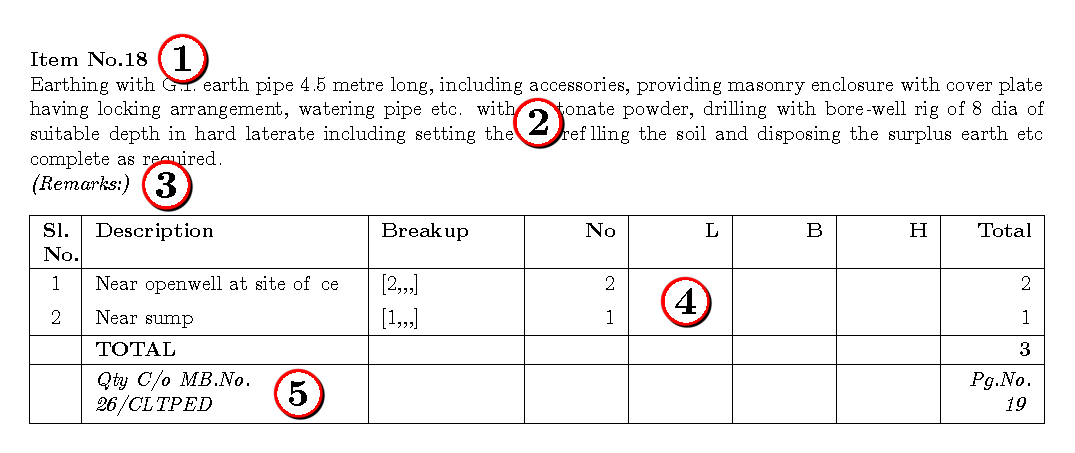
\includegraphics[width=1\linewidth]{figures/measurementstandard.pdf}
  \end{block}
  \begin{overlayarea}{\linewidth}{5\baselineskip}
      \begin{enumerate}
        \item<1|only@1> Item number as per agreement schedule or extra/substituted item schedules.
        \item<2|only@2> Description as per agreement schedule or extra/substituted item schedules
        \item<3|only@3> Any remarks about the item.
        \item<4|only@4> Tabulated list of measurements.
        \item<5|only@5> Cross reference to the abstract of measurements.
      \end{enumerate}
  \end{overlayarea}
\end{frame}

\begin{frame}
  \frametitle{Measurement Items}
  \framesubtitle{Standard Measurement Item}
  \begin{block}{How to record measurements?}
    \begin{longtabu} to \textwidth {X[1,c] X[10,l] X[5,l] X[1,r] X[1,r] X[1,r] X[1,r] X[1,r]}
		  \hline
		  \emph{Sl} & \emph{Description} & \emph{Breakup} & \emph{N} & \emph{L} & \emph{B} & \emph{H} & \emph{T} \\
		  \hline
		  \endhead
		  1 & Inside room 1 of wing 2, 2nd floor & [1,,,] & 1 &  &  &  & 1\\ 
		  2 & From SB7(Room1) to DB1(Room2) & [,1.5+15+ 1.5,,] &  & 18 &  &  & 18\\ 
		  3 & From P1(near school building) to road crossing & [,15+14,,] &  & 29 &  &  & 29\\ 
		\end{longtabu}
  \end{block}
\end{frame}

\begin{frame}
  \frametitle{Special Measurement Items}
  \framesubtitle{Multiple items}
  \begin{block}{}
    \centering
    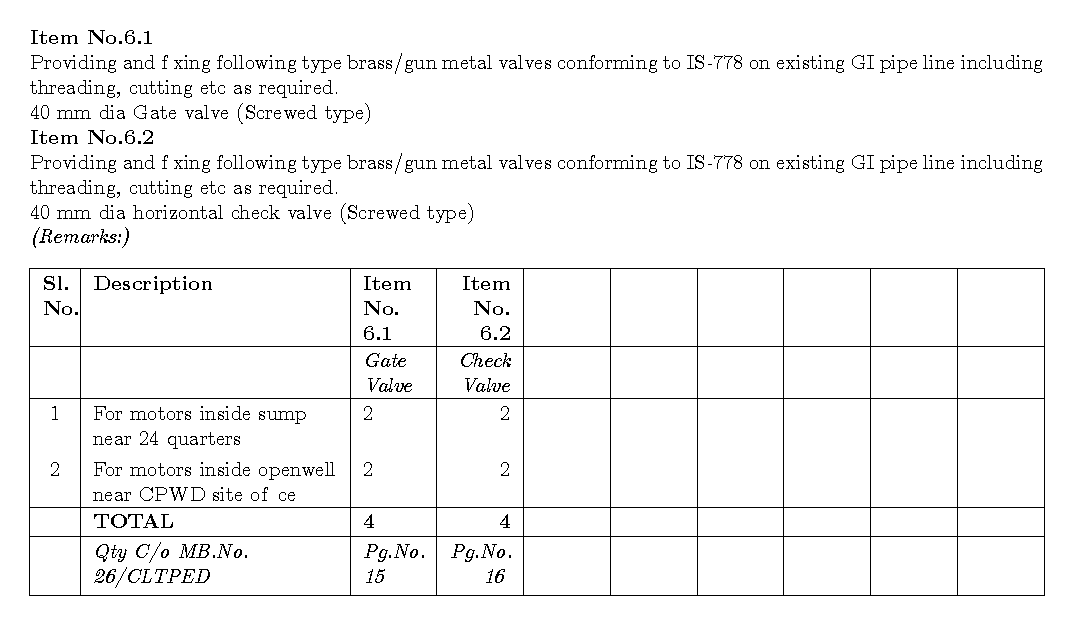
\includegraphics[width=1\linewidth]{figures/measurementNNNNNN.pdf}
  \end{block}
\end{frame}

\begin{frame}
  \frametitle{Special Measurement Items}
  \framesubtitle{Table of points}
  \begin{block}{}
    \centering
    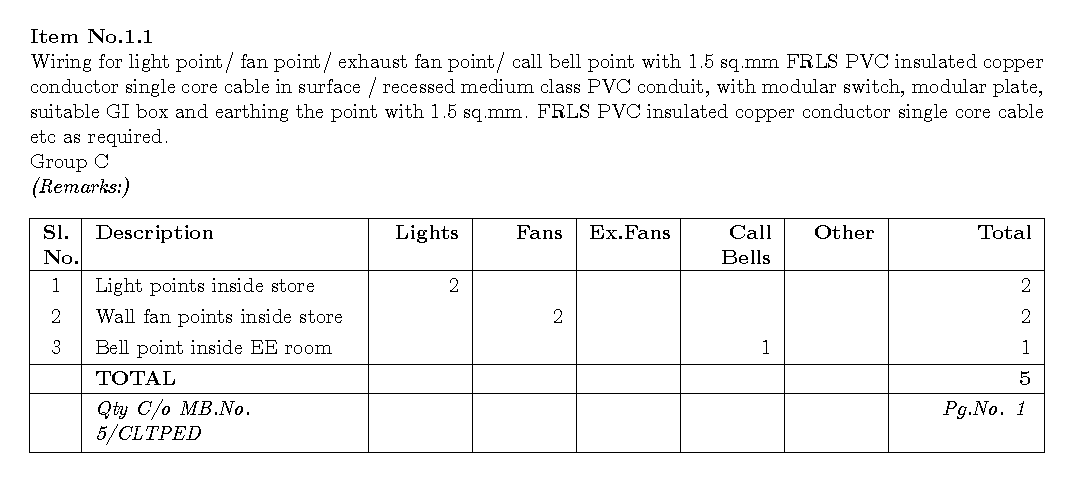
\includegraphics[width=1\linewidth]{figures/measurement_points.pdf}
  \end{block}
\end{frame}

\begin{frame}
  \frametitle{Completion certificate}
  \begin{block}{}
	 	\begin{center}
	 	  \scriptsize
	 		\bigskip
	 		\textbf{COMPLETION CERTIFICATE}
		 	\begin{longtabu}{p{.3\textwidth} c p{.5\textwidth}}
		 		Name of Work & : & \emph{\textless name of work\textgreater} \\
		 		Situation & : & \emph{\textless situation\textgreater}\\
		 		Agreement No. & : & \emph{\textless agreement number\textgreater}\\
		 		Agency & : & \emph{\textless agency}\\
		 		Date of Start & : & \emph{\textless actual date of start\textgreater}\\
		 		As per agreement & : & \emph{\textless date of start as per agreement\textgreater}\\
		 		Date of Completion & : & \emph{\textless date of completion\textgreater} \\
		 	\end{longtabu}
		 \end{center}
		 \parbox{0.9\linewidth}{\scriptsize
		 Certified that the work has been physically completed on \emph{\textbf{\textless date of completion\textgreater}} and that no defects are apparent and contractor has removed from the premises on which the work was carried out all the debris scaffolding and surplus materials and cleared off all dirt from wood work, ceiling, walls, floors and all other parts of the building up on which or about which he has been in possession for the purpose of execution thereof.
		 
		 This is however subject to measurement being recorded and quality being checked by the competent authority.
		 }
  \end{block}
\end{frame}

\begin{frame}
  \frametitle{Abstract of measurements}
  \begin{columns}
    \begin{column}{.5\textwidth}
        \begin{block}{}
        \centering
        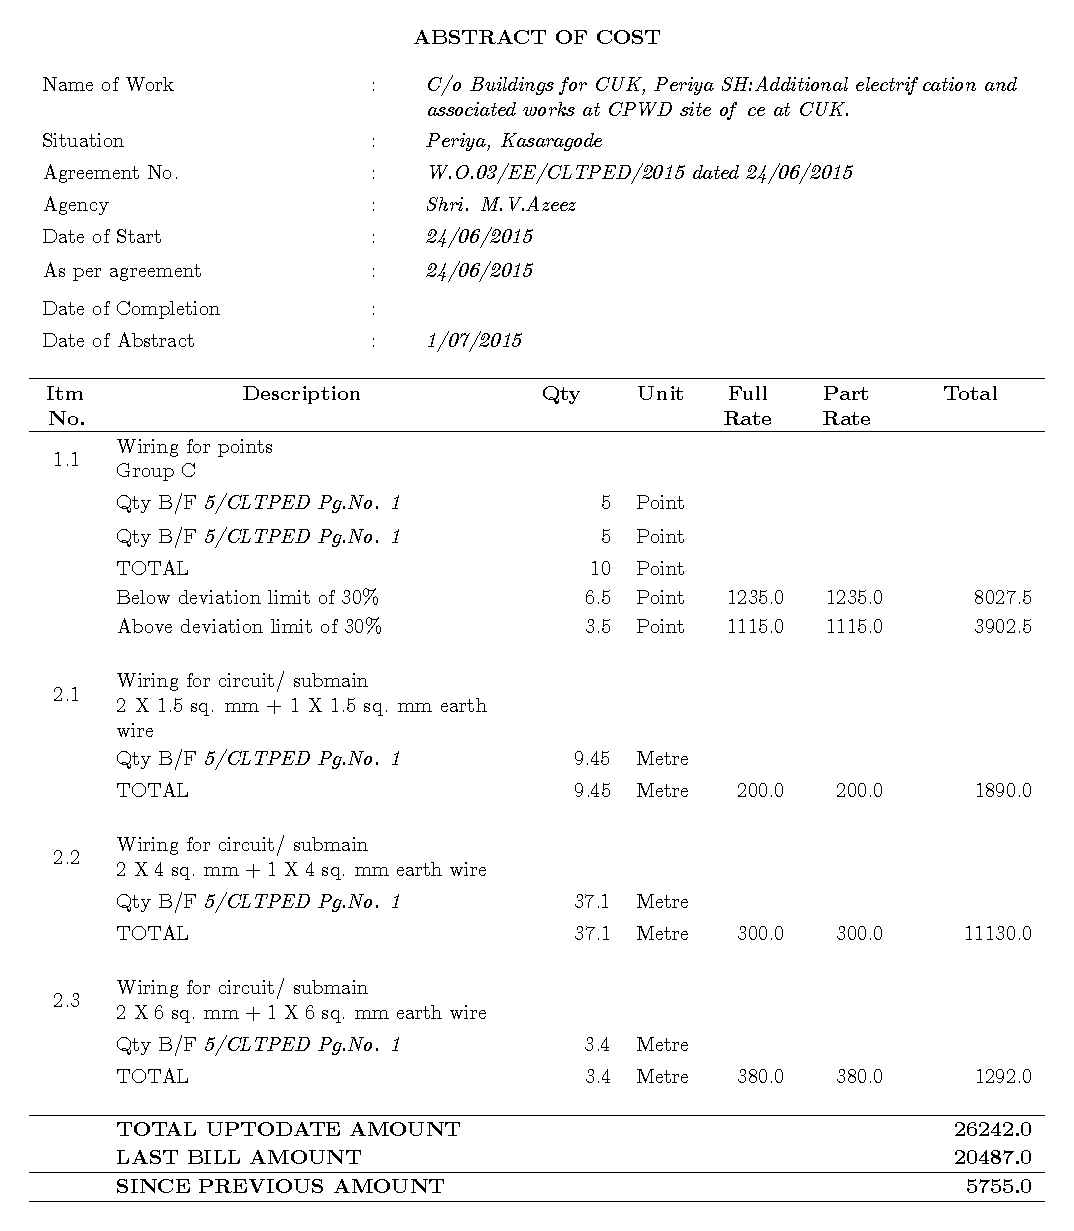
\includegraphics[width=1\linewidth]{figures/abstract.pdf}
      \end{block}
    \end{column}
    \begin{column}{.5\textwidth}
    \pause
      \begin{itemize}[<+->]
        \item Schedule/extra/substituted items appear in chronological order.
        \item Measuremnts from last bill abstract and this MB brought forward to obtain uptodate quantity.
        \item Up-to-date Total = $\sum(P.R. \times Qty)$
        \item Bill amount = Up-to-date Total - Last Bill Amount
      \end{itemize}
    \end{column}
  \end{columns}
\end{frame}

\subsection{Preperation of Bills}
\begin{frame}
  \frametitle{Preperation of Bills}
  \framesubtitle{Bill forms}
  \begin{block}{First and Final Bill}
      \begin{itemize}
        \item<2-> Prepared in CPWA-24
        \item<3-> Used when entire payment for work is made in a single bill.
      \end{itemize}
  \end{block}
  \begin{block}{Running Account Bill}
      \begin{itemize}
        \item<4-> Prepared in CPWA-26
        \item<5-> Used when payments for work are made in multiple bills.
        \item<6-> Making secured advances to contractors.
      \end{itemize}
  \end{block}
\end{frame}

\begin{frame}
  \frametitle{Preperation of Bills}
  \framesubtitle{Preparation of bill schedule}
  \begin{columns}
    \begin{column}{.5\textwidth}
        \begin{block}{}
        \centering
        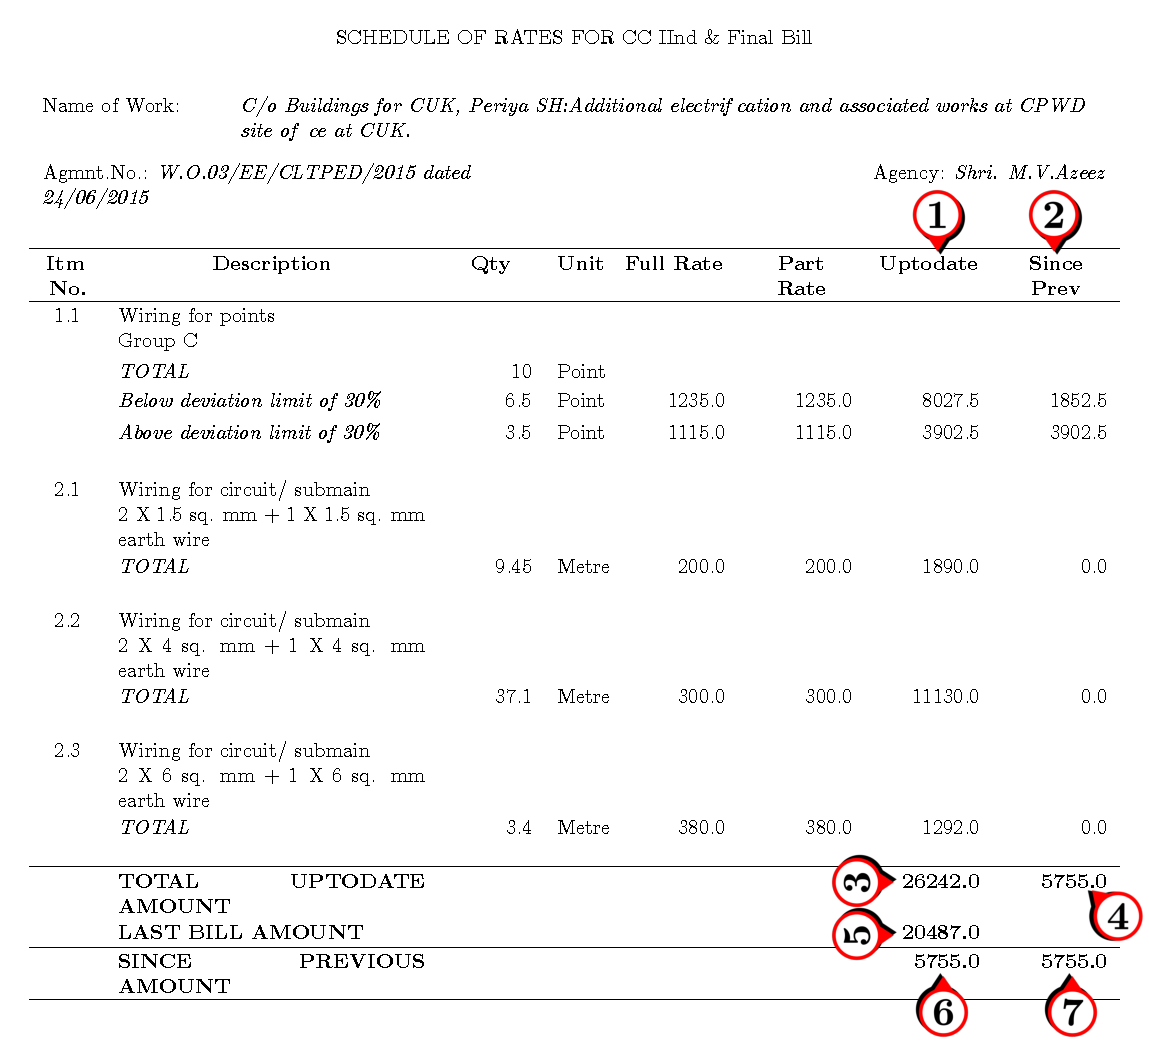
\includegraphics[width=1\linewidth]{figures/schedule.pdf}
      \end{block}
    \end{column}
    \begin{column}{.5\textwidth}
    \pause
    \begin{enumerate}[<+->]
	   	\item Quantity $\times$ Part Rate
	   	\item Column (1) of this bill - Column (1) of last bill
	   	\item Sum of Column (1)
	   	\item Sum of Column (2)
	   	\item Previous bill amount
	   	\item (5) - (3)
	   	\item (4) \\
	 \end{enumerate}
    \end{column}
  \end{columns}
\end{frame}

\section{Computerised measurements using CMB Automiser}
\begin{frame}
  \frametitle{Computerised measurements using CMB Automiser}
  \begin{block}{}
    \alert{CMB Automiser} is a computer program for preparing computerised measurement books and bills.
  \end{block}
  \pause
  \begin{block}{Features of \emph{CMB Automiser}}
    \begin{itemize}[<+->]
      \pause
      \item Generation of CMBs and abstract of cost.
      \item Generation of Bill schedule.
      \item Generation of deviation statement.
      \item Support for measurement entry in multiple formats.
      \item Fully cross referenced output.
      \item Start billing a work at the Ist or Nth bill.
    \end{itemize}
  \end{block}
\end{frame}

\subsection{Workflow}
\begin{frame}
  \frametitle{Workflow}
  \centering
  \includegraphics[width=0.8\linewidth]{figures/workflow_present.pdf}
\end{frame}

\subsection{Program Interface}
\begin{frame}
  \frametitle{Program Interface}
  \begin{columns}
    \begin{column}{0.5\textwidth}
      \centering
      \begin{tikzpicture}[every node/.style={anchor=south west,inner sep=0pt},x=1mm, y=1mm]   
        \node (fig1) at (0,0) {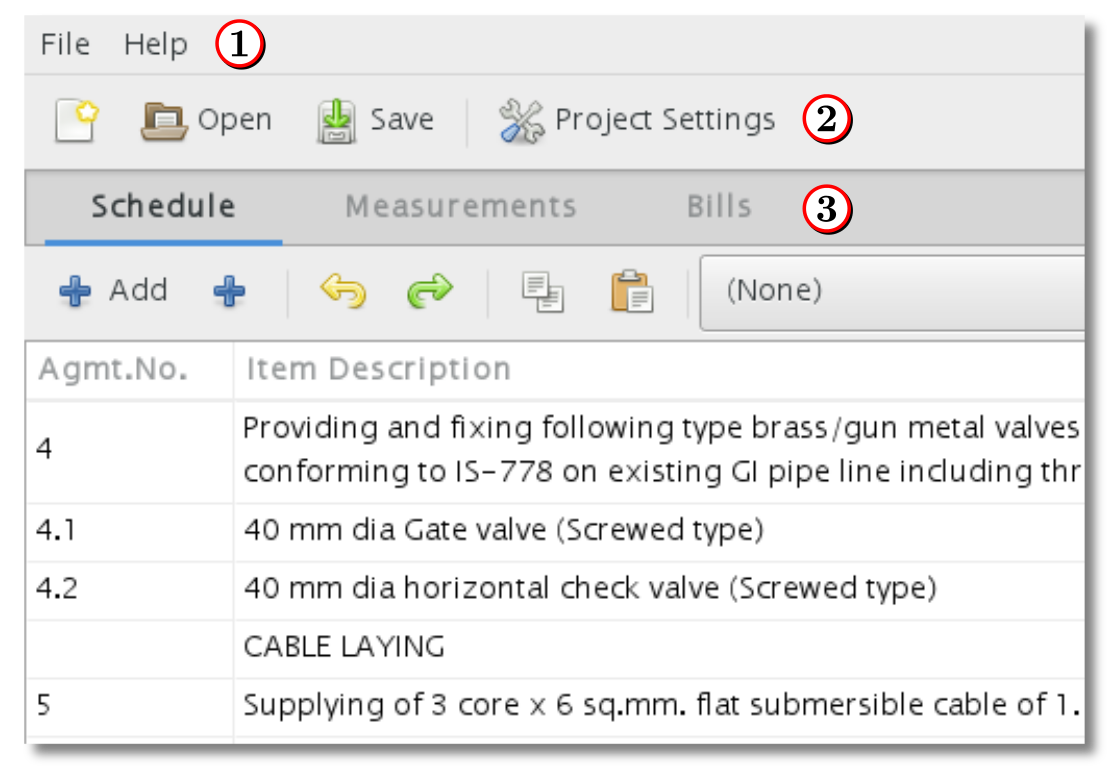
\includegraphics[width=1\linewidth]{screenshots/window_main.png}<1->};
        \node (fig3) at (5,-10) {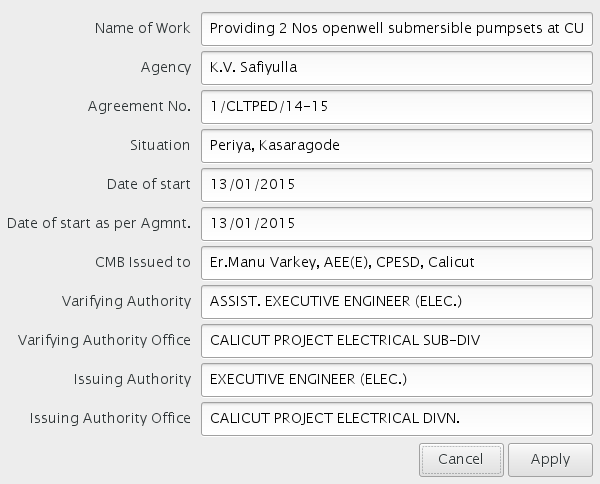
\includegraphics[width=0.8\linewidth]{screenshots/window_project.png}<4>};
      \end{tikzpicture}
    \end{column}
    
    \begin{column}{0.5\textwidth}
      \begin{itemize}
        \item Main interface is divided into three.
        \begin{enumerate}
          \item<2-> Menu Bar
          \item<3-> Tool Bar
          \item<5-> Tabs/Views
        \end{enumerate}
      \end{itemize}
    \end{column}
  \end{columns}
\end{frame}

\begin{frame}
  \frametitle{Program Interface}
  \framesubtitle{Schedule View}
    \centering
    \includegraphics[width=1\linewidth]{screenshots/window_sch_present.png}
    \pause
    \begin{columns}
      \begin{column}{0.5\textwidth}
        \begin{enumerate}[<+->]
          \item Add row
          \item Add multiple rows
          \item Select \emph{.xlsx} file for import
          \saveenum
        \end{enumerate}
      \end{column}
      \begin{column}{0.5\textwidth}
        \begin{enumerate}[<+->]
          \resume
          \item Import from selected file
          \item Delete Row
          \item Schedule items
        \end{enumerate}
      \end{column}
    \end{columns}
\end{frame}

\begin{frame}
  \frametitle{Program Interface}
  \framesubtitle{Measurements View}
    \centering
    \begin{overlayarea}{\linewidth}{11\baselineskip}
    \begin{tikzpicture}[every node/.style={anchor=north west,inner sep=0pt},x=1mm, y=1mm]   
        \node (fig1) at (0,0) {\includegraphics[width=1\linewidth]{screenshots/window_meas_present.png}<1->};
        \node (fig2) at (0,0) {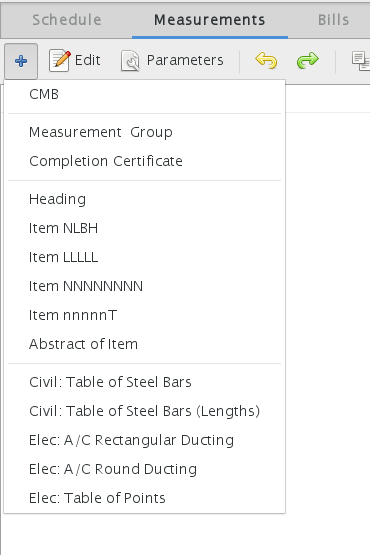
\includegraphics[width=1\linewidth]{screenshots/window_meas_menu.png}<8,15>};  
        \node (fig3) at (0,-3) {\includegraphics[width=0.8\linewidth]{screenshots/window_nlbh_meas.png}<9-13>};
        \node (fig4) at (0,-3) {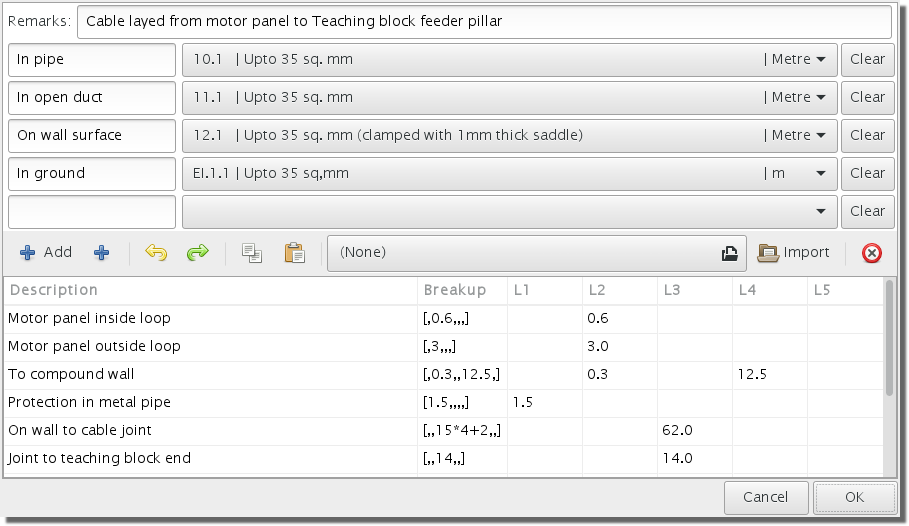
\includegraphics[width=0.8\linewidth]{screenshots/window_lllll.png}<16>};
      \end{tikzpicture}
    \end{overlayarea}
    \pause
    \begin{overlayarea}{\linewidth}{1\baselineskip}
      \begin{enumerate}
        \item<2|only@2> Add measurement item
        \item<3|only@3> Edit measurement item
        \item<4|only@4> Select output folder
        \item<5|only@5> Generate CMB
        \item<6|only@6> Delete measurement item
        \item<7|only@7> Measurement items
        \setcounter{enumi}{0}
        \item<10|only@10> Any remarks about the measurements.
        \item<11|only@11> Schedule item to be measured.
        \item<12|only@12> Breif description of the item being measured.
        \item<13|only@13> Measurement Schedule
      \end{enumerate}
    \end{overlayarea}
\end{frame}

\begin{frame}
  \frametitle{Program Interface}
  \framesubtitle{Bills View}
  \centering
  \begin{overlayarea}{\linewidth}{11\baselineskip}
  \begin{tikzpicture}[every node/.style={anchor=north west,inner sep=0pt},x=1mm, y=1mm]   
      \node (fig1) at (0,0) {\includegraphics[width=1\linewidth]{screenshots/window_bill_present.png}<1->};
      \node (fig2) at (3,-3) {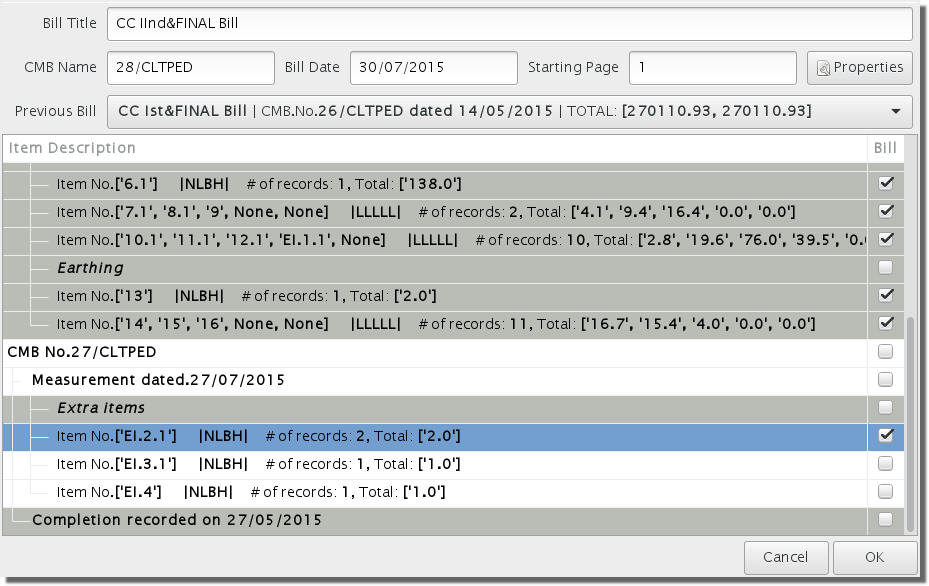
\includegraphics[width=0.8\linewidth]{screenshots/window_bill_edit.png}<9->};
      \node (fig3) at (6,-6) {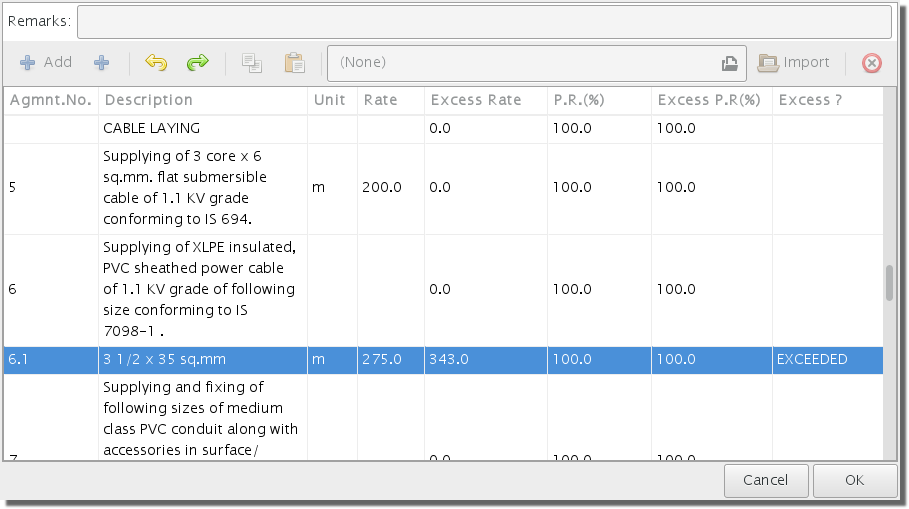
\includegraphics[width=0.8\linewidth]{screenshots/window_bill_prop.png}<10>};
    \end{tikzpicture}
  \end{overlayarea}
  \pause
  \begin{overlayarea}{\linewidth}{1\baselineskip}
    \begin{enumerate}
      \item<2|only@2> Add Bill
      \item<3|only@3> Add custom Bill
      \item<4|only@4> Edit Bill
      \item<5|only@5> Select output folder
      \item<6|only@6> Generate Bill \& CMBs
      \item<7|only@7> Delete Bill
      \item<8|only@8> Bill List
    \end{enumerate}
  \end{overlayarea}
\end{frame}

\begin{frame}
  \frametitle{Program Interface}
  \framesubtitle{Bills View - Adding a custom bill}
  \centering
  \begin{overlayarea}{\linewidth}{12\baselineskip}
  \begin{tikzpicture}[every node/.style={anchor=north west,inner sep=0pt},x=1mm, y=1mm]   
      \node (fig1) at (0,0) {\includegraphics[width=1\linewidth]{screenshots/window_bill_present.png}<1->};
      \node (fig2) at (3,-3) {\includegraphics[width=0.8\linewidth]{screenshots/window_bill_cust_edit.png}<2->};
      \node (fig3) at (6,-6) {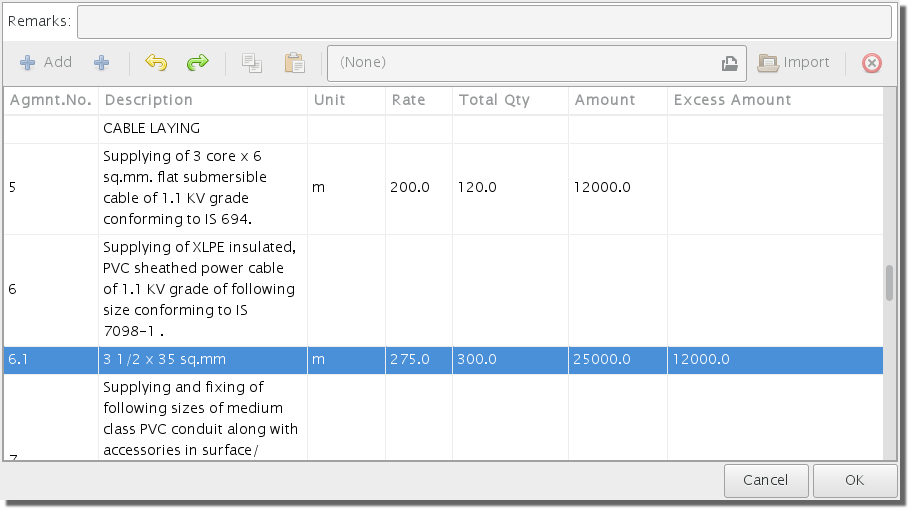
\includegraphics[width=0.8\linewidth]{screenshots/window_bill_cust_prop.png}<3>};
    \end{tikzpicture}
  \end{overlayarea}
\end{frame}

\section*{Conclution}
\begin{frame}
  \frametitle{Conclution}
  \centering
  \textbf{THANK YOU}\\
  \bigskip
  \textbf{ANY QUESTIONS ?}
\end{frame}

\end{document}
